
%%%%%%%%%%%%%%%%%%%%%%%%%%%%%%%%%%  memoria.tex %%%%%%%%%%%%%%%%%%%%%%%%%%%%%%%%%

%%%%% Memoria del Trabajo Academicamente Dirigido: Experiencias con PyCUDA %%%%%%
%%%%% Alejandro Samarin Perez - Sergio Armas Perez - Lionel A. Mena Garcia %%%%%%
\documentclass[twoside]{article}
\usepackage{fontspec}
\usepackage{xunicode}
\usepackage{xltxtra}
\usepackage{graphicx}
\usepackage{anysize}
\marginsize{3cm}{3cm}{1cm}{1cm}

\graphicspath{{imgs/}}

\usepackage{listings}
\usepackage{color}
\lstloadlanguages{Python}
\lstset{
  language=Python,                      % C,Fortran,XML
  basicstyle=\scriptsize,               % Listados en small
  keywordstyle=\color{red},             % Palabras clave en rojo
  identifierstyle=\ttfamily,
  escapeinside={(*@}{@*)},
  commentstyle=\color{blue},            % comentarios en azul
  stringstyle=\color{green},            % cadenas en verde
  showstringspaces=false,
  frame=tb,
  captionpos=t,
  belowcaptionskip=12pt,
  stepnumber=2,                                         % Opciones de lineas y etiquetas
  numberstyle=\scriptsize,
  numbersep=5pt,
  tabsize=1
}


%%%%%%%%%%%%%%%%%%%%%%%%%%%%%%%%%%%%%%%%%%%%

\begin{document}

\title{Memoria TAD:\\*Experiencias con Python y CUDA\\*en Computación de Altas Prestaciones}

\author{Sergio Armas, %
     Lionel Mena, %
     Alejandro Samarín,\\*% 
     Vicente Blanco%
     \thanks{Dpto. Estadística, I.O. y Computación, Univ. La Laguna, e-mail: {\tt vblanco@ull.es}}, %
     Alberto Morales y % 
     Francisco Almeida
}

\maketitle
% Oculta las cabeceras y los números de página.
% Ambos elemetos se añadirán durante la edición de las actas completas.
\markboth{}{}
\pagestyle{empty} 
\thispagestyle{empty} % Oculta el número de la primera página

\begin{abstract}
El aprovechamiento de la capacidad de cómputo de los dispositivos gráficos para resolver problemas computacionalmente complejos está en auge. El alto grado de paralelismo que esta arquitectura provee, además de la disponibilidad de kits especializados de desarrollo de software para el público general, abren la puerta a nuevas formas de resolver problemas científicos en una fracción del tiempo que emplearían algoritmos similares basados en CPU. El siguiente paso es encontrar el equilibrio entre la potencia de estos paradigmas de programación y la flexibilidad de los lenguajes modernos. Es aquí donde PyCUDA entra en escena; un "wrapper" de la programación CUDA para Python, de forma que ofrece al programador el acceso a la computación de altas prestaciones sobre dispositivos gráficos sin abandonar la comodidad y el dinamismo de este lenguaje (orientación a objetos, tipado dinámico, intérprete interactivo, etc.). Nuestros objetivos se centran en, por un lado, preparar una máquina de prueba equipada con el hardware necesario y, por otro, comprobar las facilidades que promete PyCUDA así como su rendimiento frente a problemas reales.
\end{abstract}

%\begin{keywords}
%   Python, CUDA, PyCUDA
%\end{keywords}

\section{Introducción}
La computación es una rama del conocimiento que está en constante evolución. Ya en la década de los 60 del pasado siglo el cofundador de Intel, Gordon E. Moore, se atrevió a postular su afamada ley por la cual cada 18 meses se duplica la capacidad de procesamiento de un circuito integrado. Esta ley ha venido cumpliéndose de manera casi asombrosa hasta nuestros días, aunque frente a la complejidad cada vez mayor que supone la integración a escala nanométrica de los componentes electrónicos se han venido imponiendo ciertos cambios de paradigma en la forma en que se hacen cálculos computacionales.

\vspace{5 mm}

Uno de los cambios más importantes ha sido la introducción del cómputo paralelo. La capacidad de procesar varios subproblemas concurrentemente permite, en teoría, obtener ganancias de rendimiento varias veces superior a una ejecución secuencial equivalente. En la práctica, la ganancia real de rendimiento estará supeditada a muchas variables, tales como lo paralelizable que sea el algoritmo en concreto que se está tratando, el grano empleado, etc. A pesar de ello, las ventajas potenciales del cálculo paralelo sobrepasan el costo del cuidado añadido con el que hay que proceder. El siguiente paso en el inexorable camino de la ley de Moore ha sido el traslado de estas operaciones paralelas de la CPU a la GPU. Tradicionalmente, las tarjetas y dispositivos gráficos han ido íntimamente ligados a la visualización de datos y programas, pero la particular arquitectura de las GPU (altamente optimizada para multiplicaciones de matrices y manejo de primitivas, por ejemplo) ha llamado la atención de la comunidad como una gran oportunidad de mejorar notablemente el rendimiento de algoritmos de propósito general, no solamente orientados a visualización gráfica como hasta el momento. 

\vspace{5 mm}

La capacidad de cómputo de las unidades de procesamiento gráfico (GPU) ha alcanzado en los últimos años un desarrollo notable que ha crecido de manera paralela a un fuerte incremento en la producción y demanda de dispositivos que las integran, tales como smartphones, tablets, etc., además de seguir presentes en tarjetas gráficas o placas base con cada vez más relevancia. Precisamente, dicho aumento de potencia ha comenzado a hacer atractivo su empleo para la manipulación de cantidades masivas de datos en ámbitos ajenos al del video tales como criptología, biología computacional, cálculo científico etc., que, por su naturaleza paralela, son susceptibles de ejecutarse con más eficiencia, incluso, que en una CPU tradicional. Esta técnica de usar la GPU en aplicaciones que tradicionalmente se habían ejecutado en CPU recibe el nombre de GPGPU (General-purpose computing on graphics processing units).

\vspace{5 mm}

NVIDIA \cite{DBLP:conf/csse/YangZP08} es, probablemente, el fabricante especializado que más ha apostado por este enfoque, desarrollando un modelo de programación denominado CUDA (Compute Unified Device Architecture), que permite ejecutar algoritmos en sus GPU. El lenguaje de programación diseñado para ello es una variación de C que contiene extensiones para trabajar con la GPU y ciertas restricciones (no permite recursividad ni punteros a funciones, solo permite números en precisión simple en la mayoría de tarjetas lanzadas al mercado hasta ahora, etc.).

\ldots utilizando PyCUDA~\cite{DBLP:journals/corr/abs-0911-3456}

y una gráfica \ref{fig:Fermi}

%%%%%%%%%%%%%%%%%%%%%%%%%%

\section{Administración de la máquina de pruebas}

Nuestro primer reto frente al TAD que nos ocupa ha sido preparar un entorno de trabajo sobre una máquina provista a tal efecto de dos tarjetas NVIDIA con capacidad CUDA. Esta máquina, que de aquí en adelante nos referiremos a ella como \emph{Garoé} (en alusión a su \emph{hostname} asignado), presenta la siguiente configuración de hardware:

\begin{description}
   \item[CPU] Intel Core i7 930 @ 2.80GHz
   \item[RAM] 4 GB Total - Kingston ValueRAM 2 GB (x2)
   \item[Disco duro] Seagate 500 GB S-ATA
   \item[Tarjeta gráfica 1] NVIDIA Tesla C2050
   \item[Tarjeta gráfica 2] NVIDIA Tesla C1060
\end{description}

Se trata, pues, de una máquina razonablemente moderna que no tiene a priori por qué representar un impedimento para el transcurso del trabajo. En cuanto al software, al momento de recibir acceso a la máquina pudimos comprobar que tenía instalado un sistema operativo GNU/Linux CentOS versión 5.5, una distribución orientada a servidores basada en Red Hat. Sin embargo, para nuestra labor necesitábamos de bastante software adicional; teniendo en cuenta que los repositorios disponibles de CentOS

%%%%%%%%%%%%%%%%%%%%%%%%%%

\section{Modelo de programación CUDA}

El diseño de CUDA tiene como el objetivo el desarrollo de software que de manera transparente escale el paralelismo de manera que se pueda aprovechar el incremento del numero de procesadores al tiempo que mantiene una una baja curva de aprendizaje para los programadores familiarizados con lenguajes estándares como el C.

Para lograr esto fundamentalmente posee tres puntos claves:

\begin{itemize}
   \item Jerarquía de hilos
   \item Jerarquía de memorias
   \item Sincronizaciones por Barrera
\end{itemize}

\subsection{Jerarquía de Hilos}

Se define en base a 3 elementos: hilo, bloque y grid. Estas abstracciones permiten un granulado fino del paralelismo de los datos y los hilos.

Por conveniencia, cada hilo se identifica por un vector de tres componentes (x, y, z) denominado threadIdx, así los hilos pueden identificados por un índice threadIdx unidimensional, bidimensional o tridimensional, formando a su vez un bloque unidimensional, bidimensional o tridimensional. Esto provee de una manera natural de realizar cálculos sobre elementos tales como un vector o una matriz.

Insertar imagen ThreadHierarchy.png (Figura 1)

\subsection{Jerarquía de Memoria}

Los hilos en CUDA pueden acceder a distintas memorias, unas compartidas y otras privadas. En primer lugar tenemos la memoria local privada de cada hilo. Cada bloque de hilos posee memoria compartida visible solo por los hilos del bloque y con el mismo tiempo de vida del bloque. Finalmente cada hilo en cada bloque de cada grid puede acceder a la memoria global.

Insertar imagen MemoryHierarchy.png (Figura 2)

Adicionalmente existen dos espacios de memoria de sólo lectura accesible por todos los hilos: la memoria de texturas y la memoria de constante, optimizadas para usos específicos. Las memorias global, de textura y constante persisten mientras el kernel permanezca en acción.

Asi como se puede identificar los hilos dentro de un bloque, se pueden identificar los bloques dentro de un grid, mediante una variable blockIdx que también puede ser un índice unidimensional, bidimensional o tridimensional.

\subsection{Sincronizaciones por Barrera}

Como los distintos hilos colaboran entre ellos y pueden compartir datos, se requieren de directivas de sincronización. En CUDA se puede especificar una sincronización del tipo barrera, en la que todos los hilos esperan a que los demás lleguen al mismo punto.

\subsection{Kernel}

CUDA extiende el lenguaje permitiendo definir funciones llamadas kernels, que cuando son invocadas, son ejecutadas N veces en paralelo por N diferente hilos de CUDA.

Estas abstracciones permiten un granulado fino en el paralelismo de los datos y los hilos. Conduciendo al programador a dividir el problema en subproblemas que pueden ser tratados independientemente y en paralelo por bloques de hilos, y su vez dividir estos subproblemas en elementos individuales que pueden ser resueltos en paralelo y de manera cooperativa por todos los hilos de un mismo bloque.

Esta estructura preserva la expresividad del lenguaje permitiendo que los hilos cooperen en la resolución de cada subproblema, y al mismo tiempo permite la escalabilidad. En efecto, cada bloque de hilos puede ser programado en cualquier núcleo de procesamiento que este disponible, en cualquier orden, concurrente o secuencialmente. Por lo que cualquier programa CUDA ya compilado puede ejecutarse en sistemas con distinto numero de núcleos de procesamiento como se ilustra en la figura 3, y solo el sistema de tiempo de ejecución debe conocer el numero de núcleos físicos.

Insertar imagen MemoryHierarchy.png (Figura 3)

Todo esto desde el punto de vista del programador consiste en la extensión del lenguaje con un conjunto reducido de instrucciones, lo que supone un curva de aprendizaje suave.

%%%%%%%%%%%%%%%%%%%%%%%%%%%

\begin{figure}
	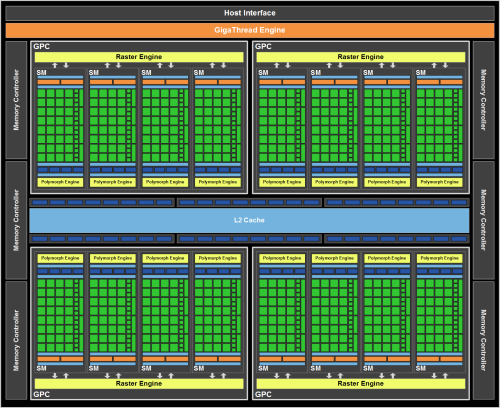
\includegraphics[width=.45\textwidth]{block_diagram_Fermi}
	\caption{\label{fig:Fermi} Diagrama de bloques de una GPU Tesla M2070 (Fermi)}
\end{figure}

y un código \ref{code:filter}

\lstinputlisting[%
   float=t,
   caption={Codigo de filtros en Python},
   label={code:filter} 
   ]%
   {code/filter.py}

\bibliographystyle{Jornadas}
\bibliography{memoria}

\end{document}

